
% ====================================
% chapter 2
% ====================================

\chapter{BinaryConnectによる良否判定}

\section{Neural Network}
Neural Networkとはニューロンと呼ばれる人間の脳細胞をもとに作られた数理モデルである.入力に対し重みをかけた時の出力から入力の特徴を抽出し分類問題を解く機械学習の1種である.

\subsection{Neural Networkの構造}
ニューラルネットワークはユニットと呼ばれる最小要素を持ち,それに対し複数の入力と重み,バイアスから計算結果を出力する.
これらは図\ref{fig_NN1}のような構造をしており,入力$x_i$に対し重み$w$を乗算したものにバイアス$b$を足すことで出力$y$を得る.計算式は以下のように表される.
\begin{align*}
y &= w_{1}x_{1} + w_{2}x_{2} + w_{3}x_{3} + b
\end{align*}
\begin{figure}[]
  \begin{center}
    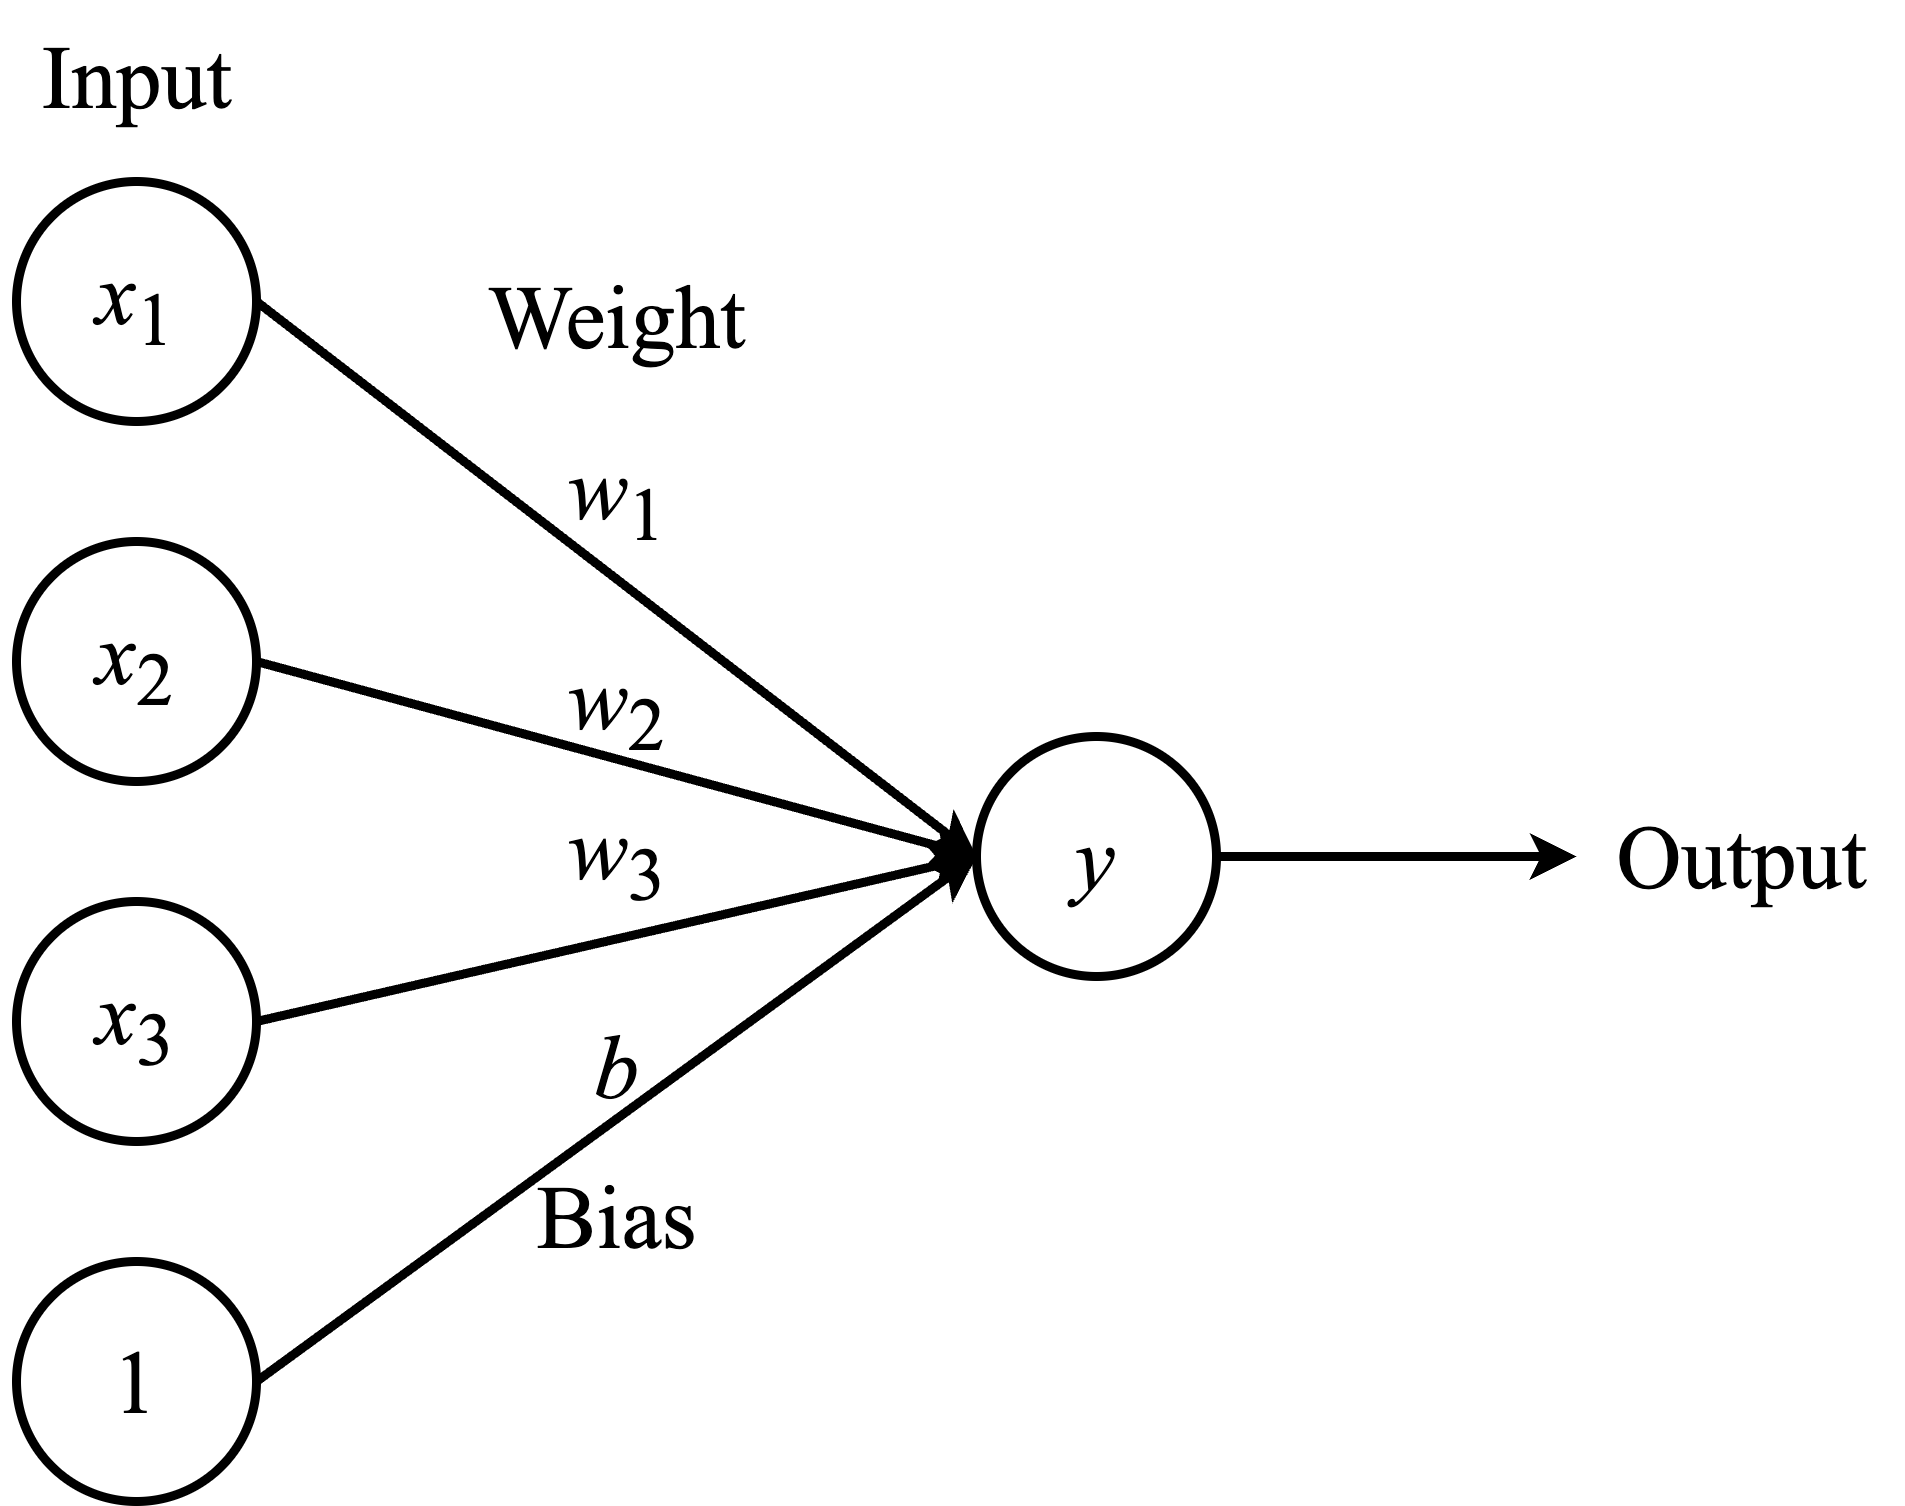
\includegraphics[scale = 0.1]{./chapter2/nn_1.png}
    \caption{ユニットの構造}
    \label{fig_NN1}
  \end{center}
\end{figure}

ここで出力$y$を複数個にすると,図\ref{fig_NN}のような構造になる.ユニットの縦方向の集まりのことを層(layer)と呼び,Neural Networkはこのlayerを複数組み合わせ,入力層・中間層・出力層という層を形成し計算を行う.
入力層$x$のユニットの個数を$i=1,2,3\ldots I$,中間層$z$のユニットの個数を$j=1,2,3\ldots J$とすると,それぞれの重みは$w_{ji}$,バイアスは$b_j$となるため一般化した計算式は以下のようになる.
\begin{figure}[]
  \begin{center}
    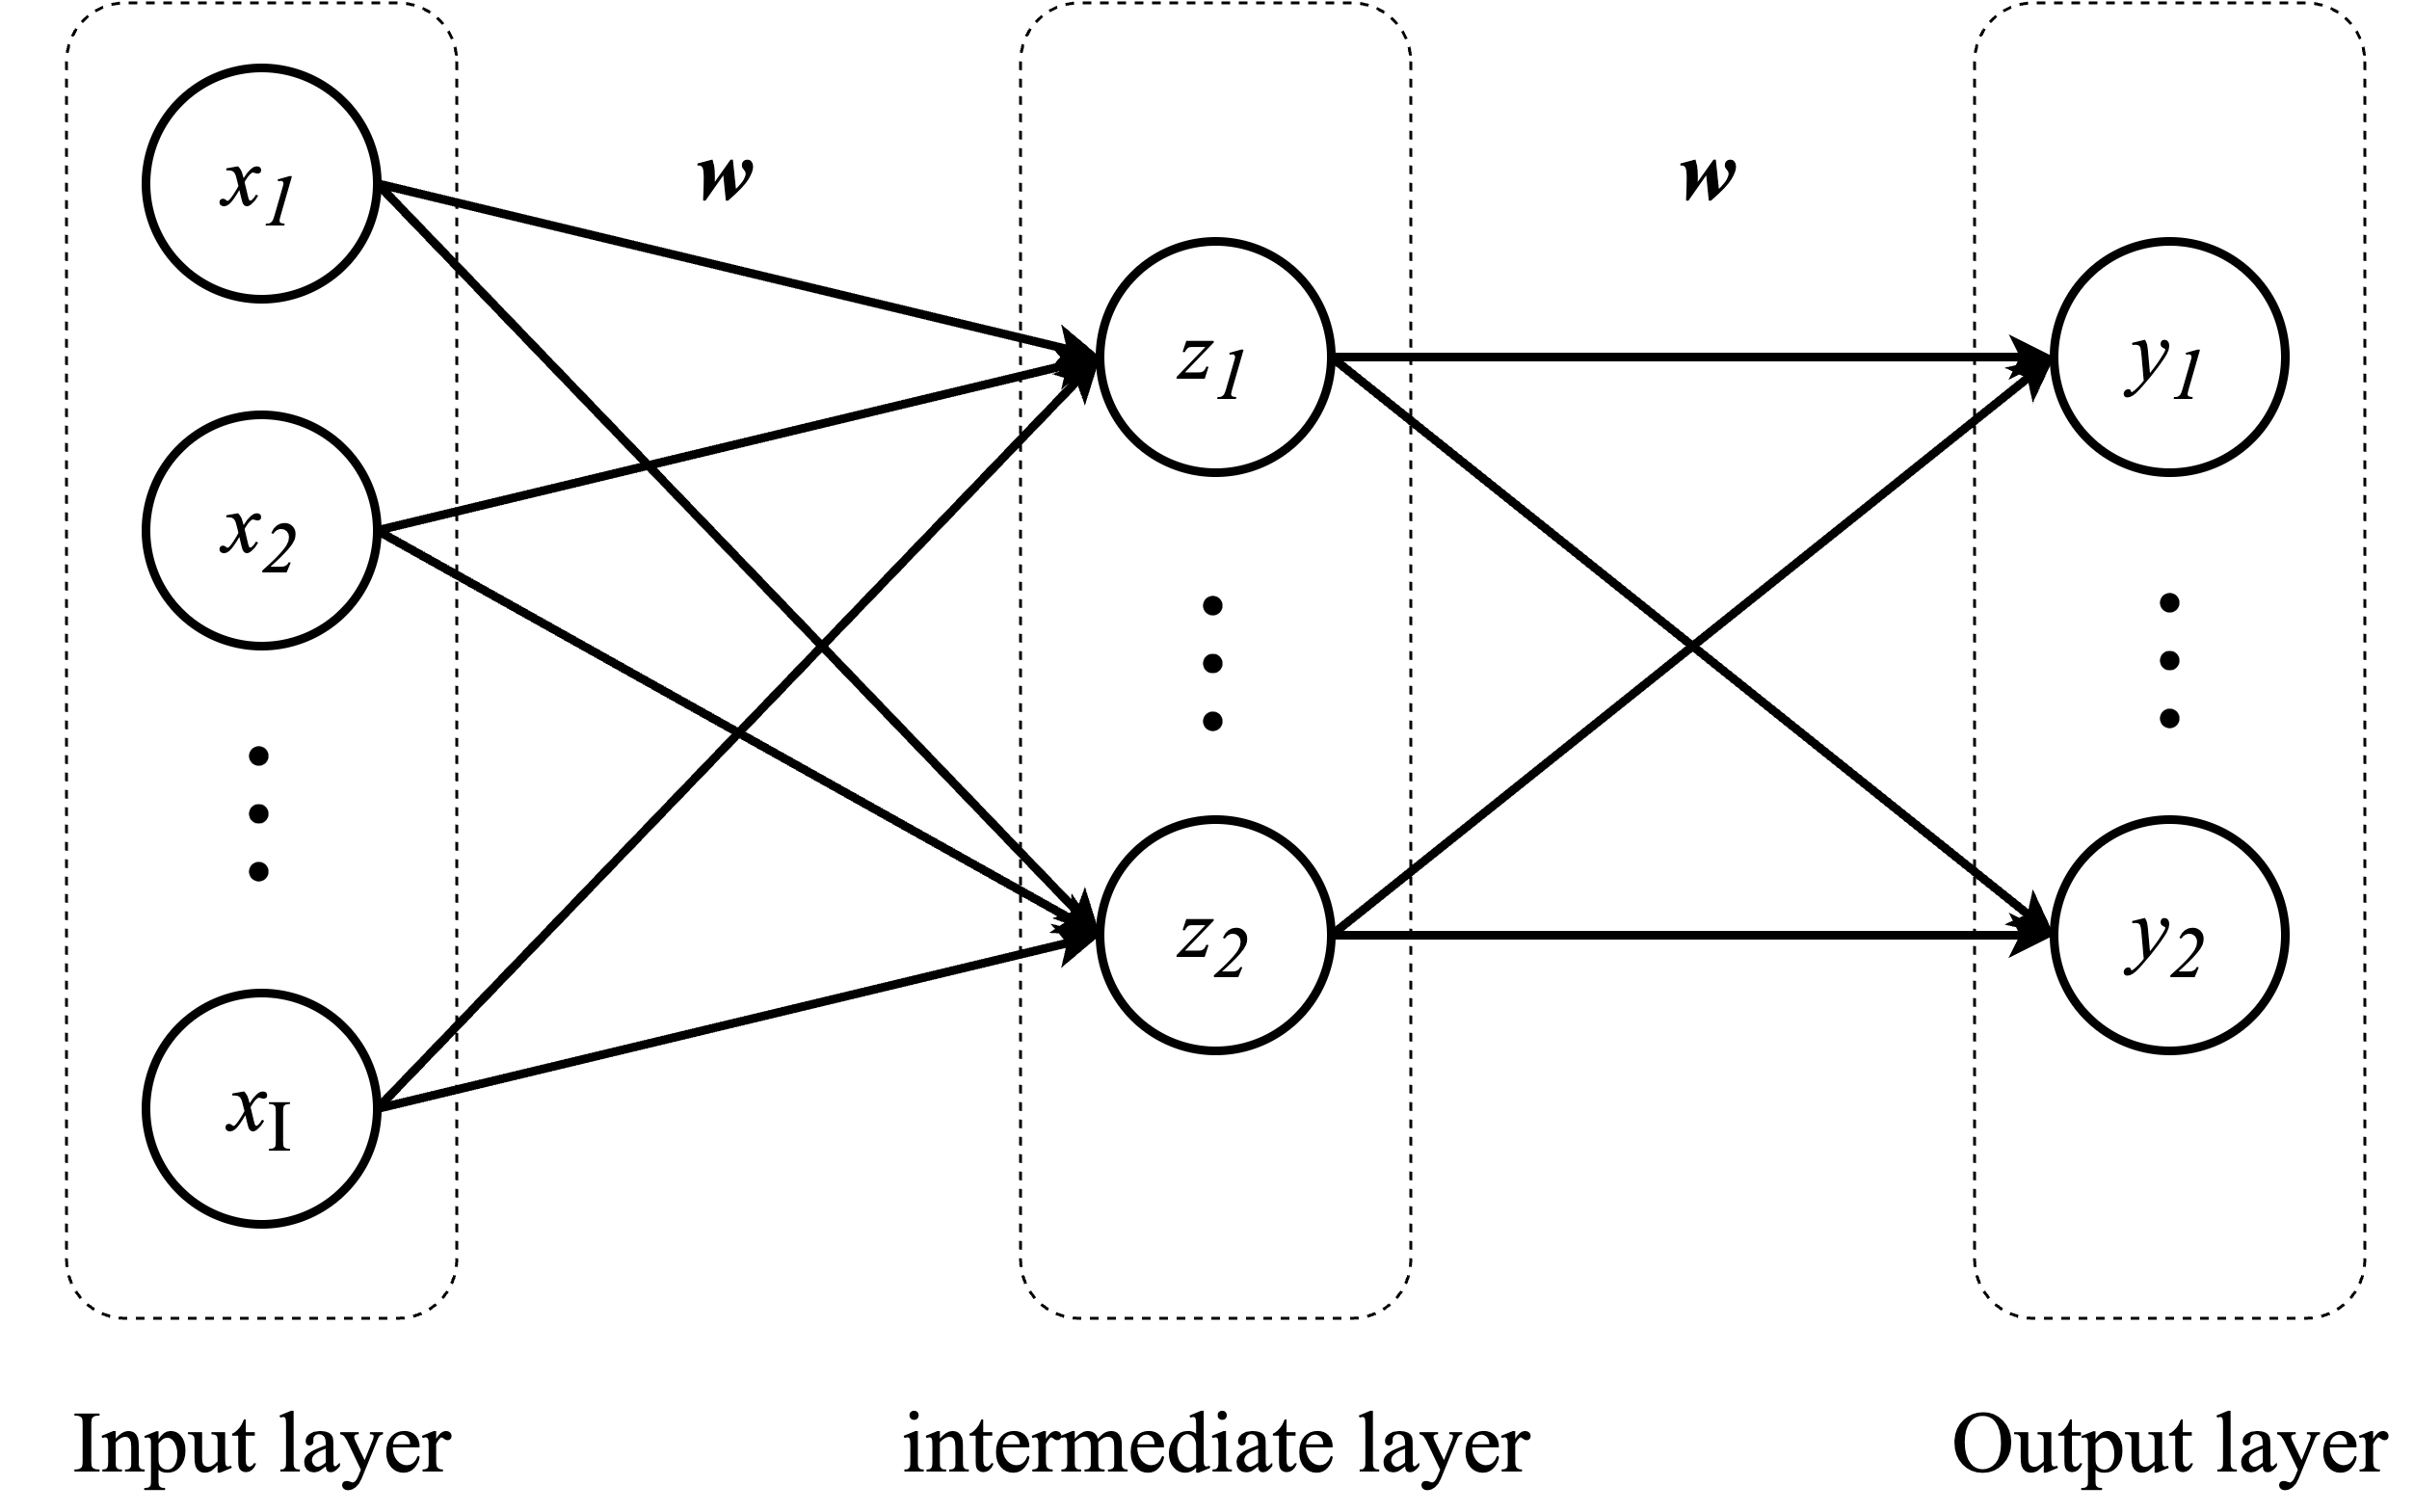
\includegraphics[scale = 0.1]{./chapter2/neural_network.png}
    \caption{Neural Networkの構造}
    \label{fig_NN}
  \end{center}
\end{figure}

\begin{align*}
z_{1} &= w_{11}x_{1} + w_{12}x_{2} + w_{13}x_{3} + b_1\\
z_{2} &= w_{21}x_{1} + w_{22}x_{2} + w_{23}x_{3} + b_2\\
z_{3} &= w_{31}x_{1} + w_{32}x_{2} + w_{33}x_{3} + b_3
\end{align*}

構造は学習モデルによって異なるため,必ずこのような形になるわけではない.そこで,入力の個数をI個とし,各要素をベクトルと行列を用いて表し,次の層のユニットへの出力を一般化すると以下のような式となる.
\begin{align*}
\bm{z} = \bm{W}\bm{x} + \bm{b}
\end{align*}

中間層は1層のみである必要はなく,中間層の出力を次の層への入力として扱うことで層を多数化し,入力層から出力層までに多数の隠れ層を追加する.層数$L$のネットワークが存在する時,$l+1$層のユニットの出力$\bm{z}^{(l+1)}$は$l$層のユニットの出力$\bm{z}^{(l)}$から計算されるため,
\begin{align*}
\bm{z}^{(l+1)} = \bm{W}^{(l+1)}\bm{z}^{(l)} + \bm{b}^{(l+1)}
\end{align*}
という式で一般化される.したがって$l=1,2,3\ldots L-1$までの計算を順に行なっていくことで各層の出力を得ることができ,最終的な出力$\bm{y}=\bm{z}^{(L)}$を計算することができる.

\subsection{学習の概要}
前項のような計算を行うと,入力が与えられたときの出力を得ることができるとわかるが,このときの出力がNeural Networkが導いた推論になるのである.教師あり学習の場合入力に対し求められる出力が正解として与えられる.その正解と,入力からネットワークによって求められた推論を比較し,より求められる正解に推論が近づくように重みを更新していくのである.

例えば$0 \ldots 9$までの手書き文字が入力として与えられその分類を行いたいとき,ネットワークの出力は$y_0 \ldots y_9$までの10個の出力を用意する.10個の出力に対し0から9までの数字を対応させ出力が1になった数字を推論として扱う.その時の構造を図\ref{fig_study}にしめす.
\begin{figure}[]
  \begin{center}
    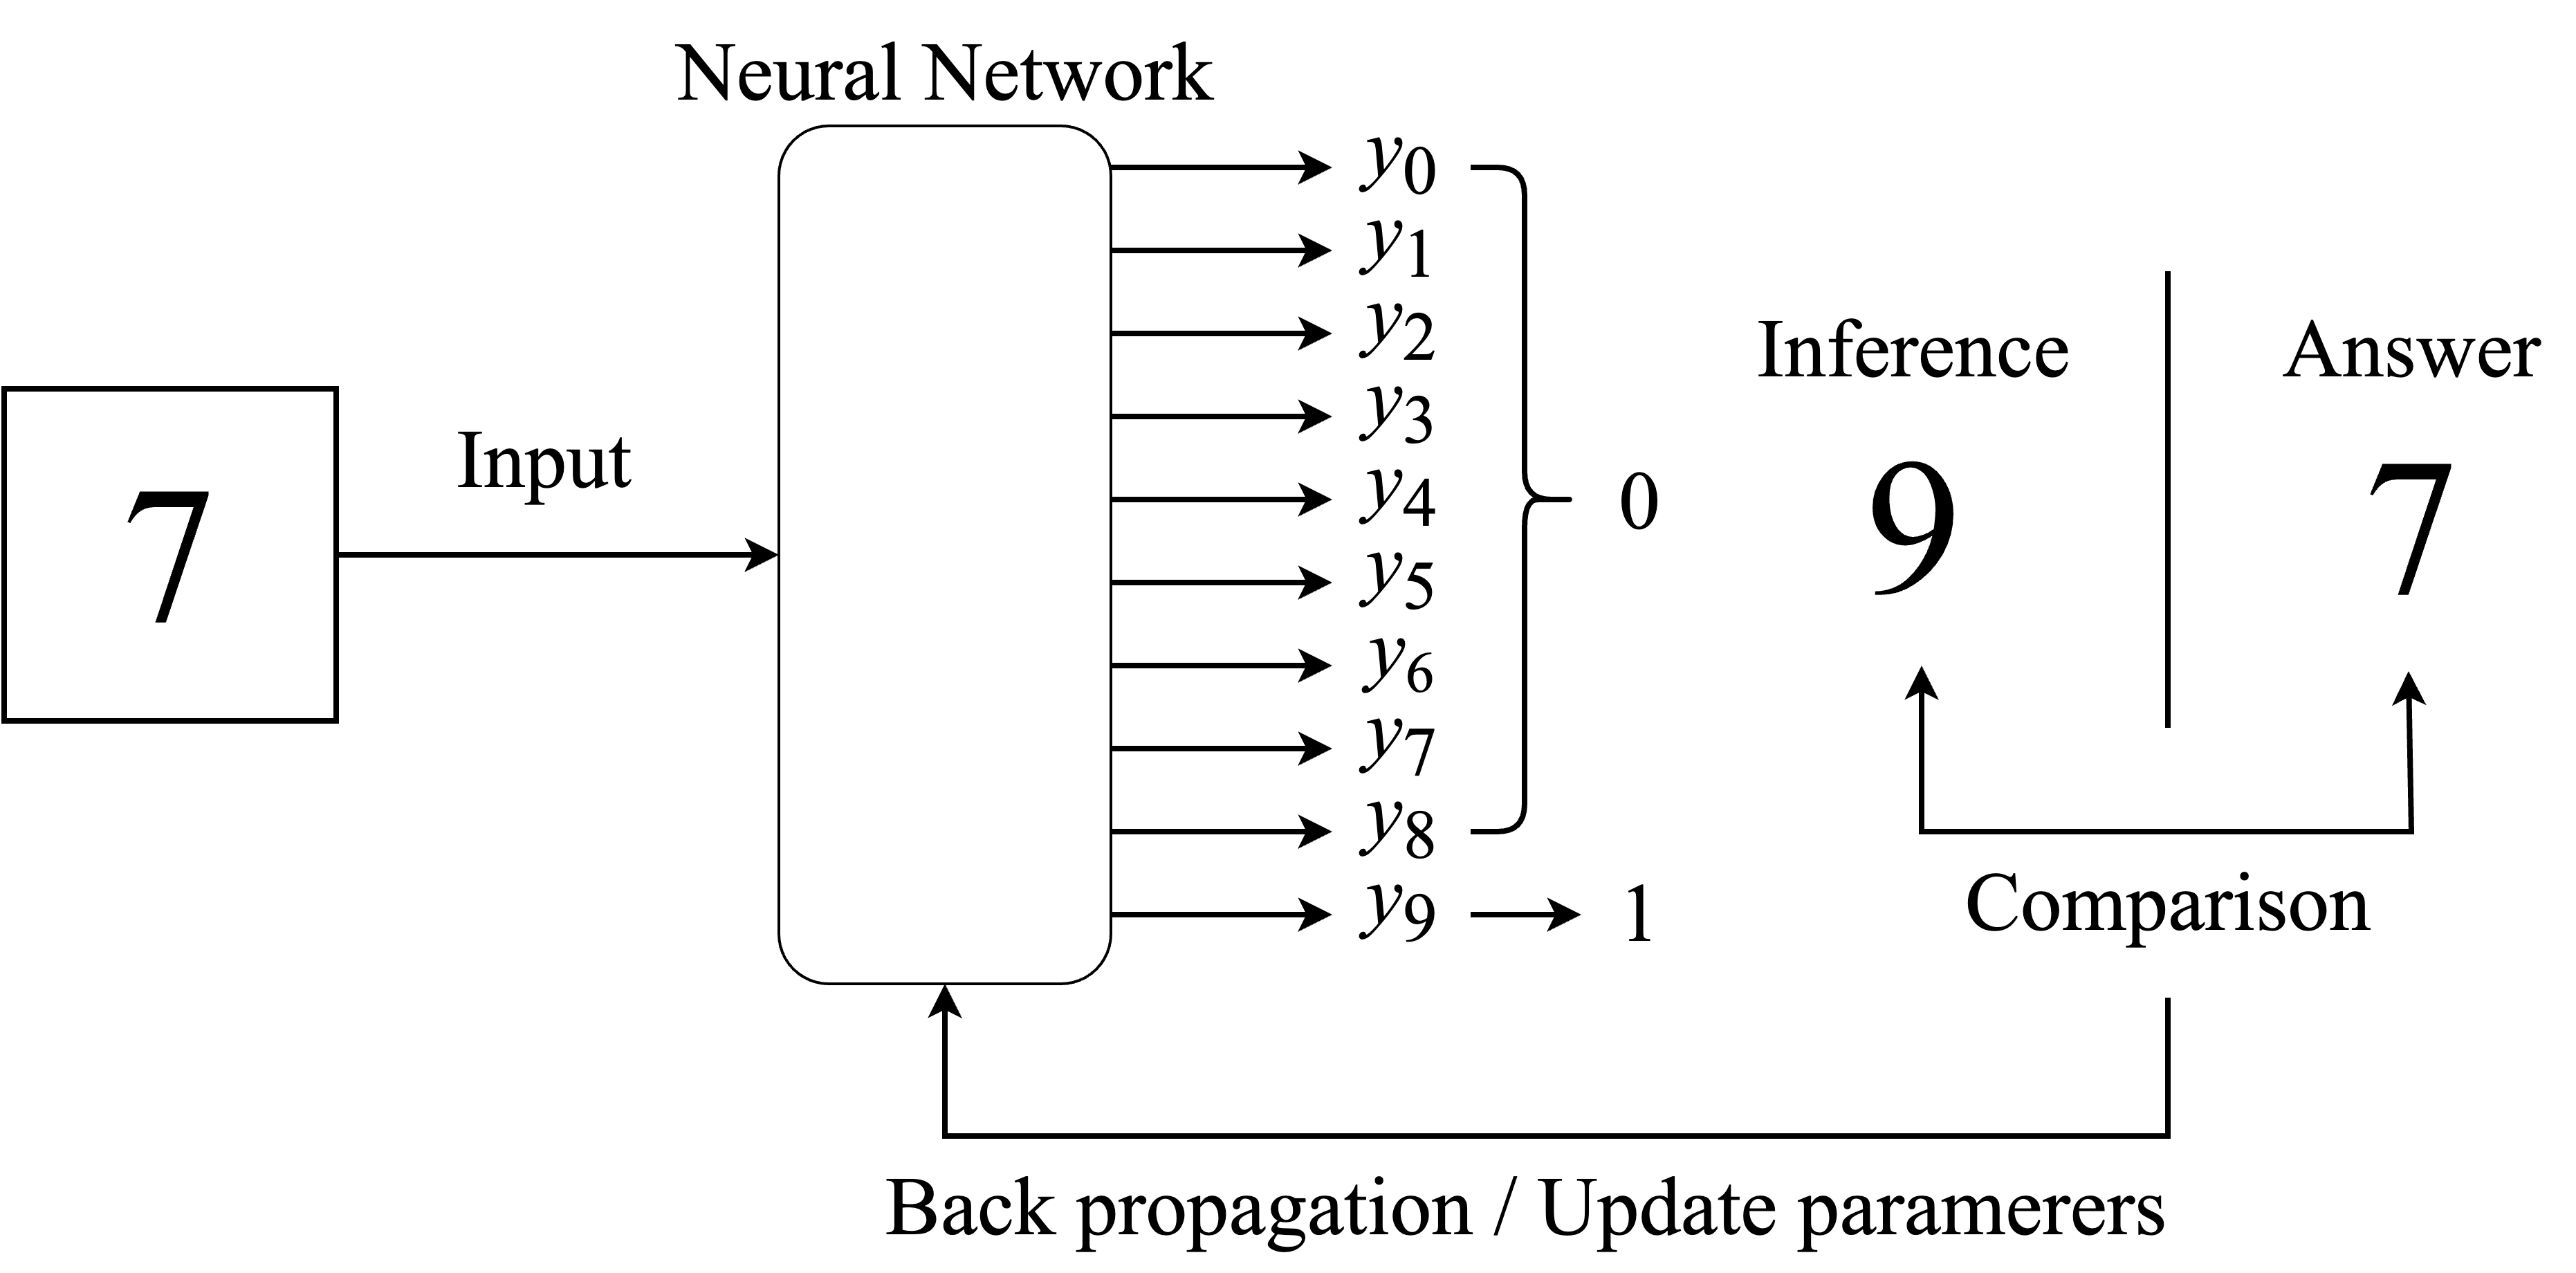
\includegraphics[scale = 0.1]{./chapter2/NN_study.png}
    \caption{学習の流れ}
    \label{fig_study}
  \end{center}
\end{figure}

このとき,実際の答えは7だが推論の結果は9となり不正解になる.そこで両者を比較し誤差逆伝搬を行うことでNeural Network内の重みをどのように変更すれば推論を正解に近づけることができるかを求める.そして重みを更新していき推論が正解に近づいていくように変更していくのがNeural Networkにおける機械学習である

\section{CNN}

\section{BinaryConnect}

